\documentclass[11pt,a4paper]{article}

\usepackage[utf8]{inputenc}
\usepackage[T1]{fontenc}
\usepackage[margin=1in]{geometry}
\usepackage[table]{xcolor}
\usepackage[most]{tcolorbox}
\usepackage{hyperref}
\usepackage{tabularx}
\usepackage{booktabs}
\usepackage{tikz}
\usepackage{fancyhdr}
\usepackage{fontawesome5}
\usepackage{amsmath}
\usepackage{graphicx}
\usepackage{float}
% --- Premium Typography & Spacing ---
\usepackage{mathpazo}
\usepackage{setspace}
\setstretch{1.15}

% --- Premium Section Headings ---
\usepackage{titlesec}
\titleformat{\section}
  {\normalfont\Large\bfseries\color{dpiblue}}{\thesection}{1em}{}[{\color{dpicloud}\vspace{0.2cm}\titlerule[1pt]}]
\titleformat{\subsection}
  {\normalfont\large\bfseries\color{dpiteal}}{\thesubsection}{1em}{}

% --- Premium Hyperlinks ---
\hypersetup{
    colorlinks=true,
    linkcolor=dpiblue,
    filecolor=dpiblue,      
    urlcolor=dpiteal,
    citecolor=dpiblue
}

% Custom Header Style
\pagestyle{fancy}
\setlength{\headheight}{25pt}
\fancyhf{}
\fancyhead[L]{\raisebox{-0.2\height}{
\includegraphics[height=15pt]{logo.png}}\hspace{0.2cm}\textbf{\color{dpiblue} DPI-LS Framework}}
\fancyhead[R]{\color{dpiblue} Measuring Quality (Q)}
\fancyfoot[C]{\color{dpiblue}\textbf{Page \thepage}}
\renewcommand{\headrulewidth}{1pt}
\renewcommand{\headrule}{\hbox to\headwidth{\color{dpiblue}\leaders\hrule height \headrulewidth\hfill}}
\usetikzlibrary{shapes.geometric, arrows.meta, positioning, calc, backgrounds, fit, trees, mindmap, matrix, shadows}

% Define DPI-LS Brand Colors
\definecolor{dpiblue}{HTML}{2b3a67}
\definecolor{dpigreen}{HTML}{498467}
\definecolor{dpired}{HTML}{b0413e}
\definecolor{dpilight}{HTML}{e5f9e0}
\definecolor{dpicloud}{HTML}{f4a261}
\definecolor{dpiteal}{HTML}{318281}

% Define Custom GitHub-Style Alerts
\newtcolorbox{dpinote}[1][]{enhanced, colback=blue!5!white, colframe=dpiblue, title={\textbf{\faInfoCircle\ NOTE}}, fonttitle=\bfseries, attach boxed title to top left={xshift=5mm,yshift=-2mm}, #1}
\newtcolorbox{dpiimportant}[1][]{enhanced, colback=red!5!white, colframe=dpired, title={\textbf{\faExclamationTriangle\ IMPORTANT}}, fonttitle=\bfseries, attach boxed title to top left={xshift=5mm,yshift=-2mm}, #1}
\newtcolorbox{dpitip}[1][]{enhanced, colback=dpigreen!5!white, colframe=dpigreen, boxrule=0.5pt, leftrule=3pt, sharp corners, #1}

\begin{document}

\begin{titlepage}
    \pagecolor{dpiblue}
    \color{white}
    \begin{center}
        \vspace*{1.5cm}
        
\includegraphics[width=6cm]{logo.png} \\[1.5cm]
        
        {\Huge \textbf{Measuring Quality}} \\[0.7cm]
        {\LARGE \textbf{Guide for the DPI-LS Project}}
        
        \vspace{2cm}
        
        {\color{dpicloud}\rule{0.5\textwidth}{1.5pt}}
        
        \vspace{2cm}
        
        {\Large \textit{Digital Performance Index --- Quality Dimension (Q)}} \\[1cm]
        
        {\large Accuracy, Consistency \& Hallucination Tracking}
        
        \vfill
        
        % Stylish Geometric Cover Overlay
        \begin{tikzpicture}[remember picture, overlay]
            \fill[white, opacity=0.05] (current page.north east) circle (5cm);
            \fill[white, opacity=0.05] (current page.south west) circle (7cm);
            \fill[dpiteal, opacity=0.1] (current page.south east) circle (9cm);
            
            % Giant faded icon in the center as a watermark
            \node[font=\fontsize{150}{150}\selectfont, text=white, opacity=0.03] at (current page.center) {\faCheckDouble};
        \end{tikzpicture}
        
        \renewcommand{\arraystretch}{1.3}
        \begin{tabular}{rl}
            \textbf{Framework:} & Digital Performance Index (DPI-LS) \\
            \textbf{Dimension:} & Quality (Q) --- Weight: 20\% \\
            \textbf{Version:} & 2.5 (Extended Enterprise Edition) \\
            \textbf{Status:} & Architectural Reference \\
        \end{tabular}
        
        \vspace{2cm}
        
        {\color{dpicloud}\rule{0.5\textwidth}{1pt}} \\[0.5cm]
        
        {\large DPI-LS Architecture Team}
        
        \vspace{0.3cm}
        {\normalsize Document Developed by \textbf{Malkapurapu Sivamanikanta}}
        
        \vspace*{1cm}
    \end{center}
\end{titlepage}
\pagecolor{white}
\color{black}

\tableofcontents
\newpage

\section{Executive Summary \& Introduction}

\begin{dpinote}
The \textbf{Digital Performance Index (DPI-LS)} framework quantifies AI agent performance across 7 distinct dimensions. Within this framework, the \textbf{Quality (Q)} dimension evaluates the correctness, consistency, and reliability of the agent's output.
\end{dpinote}

Measuring the quality of non-deterministic LLM output is one of the most challenging aspects of modern FinOps and AI Governance. Unlike simple latency or unit costs, "Quality" is subjective. Does the model hallucinate facts? Is it consistent when asked the same question twice?

This document outlines the architecture for the \textbf{Quality} dimension, explaining its mathematically rigorous evaluation framework (70\% Accuracy, 20\% Consistency, 10\% Hallucination Rate) and how the DPI-LS Engine seamlessly falls back to Human-in-the-Loop Subject Matter Experts (SMEs) when automated "LLM-as-a-Judge" metrics are insufficient.

\vspace{0.5cm}

% ---------------------------------------------------------
% 2. THE ANALOGY
% ---------------------------------------------------------
\section{The SME \& LLM-Judge Analogy}

\begin{tcolorbox}[enhanced, colback=dpiblue!5!white, colframe=dpiblue, title={\textbf{\faLightbulb\ The Automated Teacher Analogy}}, fonttitle=\bfseries, boxrule=1pt, arc=2mm, drop shadow]
\textbf{\color{dpiblue}\faGraduationCap\ The Test and the Teacher:} 
Imagine a classroom where students (the AI Agents) are constantly turning in essays (outputs). To grade 10,000 essays a minute, the school hires an automated grading robot (LLM-as-a-Judge). The robot checks for three things: 
1. \textbf{Accuracy (70\%):} Did the student get the right answer?
2. \textbf{Consistency (20\%):} Does the student contradict themselves?
3. \textbf{Hallucination (10\%):} Did the student invent a fake historical event?

\vspace{0.2cm}
\textbf{\color{dpired}\faUserTie\ The Principal (Human SME):}
However, if the student writes a highly complex, nuanced essay about advanced quantum mechanics, the robot might get confused and return a \texttt{None} score. When this happens, the robot hands the essay directly to the Principal (a human Subject Matter Expert). The Principal manually grades the essay, ensuring that complex outputs are always judged accurately rather than being arbitrarily failed by the machine.
\end{tcolorbox}

\newpage

% ---------------------------------------------------------
% 3. THE MATHEMATICS OF QUALITY
% ---------------------------------------------------------
\section{The Mathematics of Quality}

The DPI-LS Engine treats the Quality score as a composite metric of three sub-metrics. All inputs must be normalized floats between \texttt{0.0} and \texttt{1.0}.

\subsection{The Quality Equation}

The total Quality ($Q$) is calculated as:

\vspace{0.5cm}
\begin{tcolorbox}[colback=dpilight, colframe=dpigreen, title=\textbf{DPI-LS Quality Formula}]
\[ Q = (0.7 \times \text{Accuracy}) + (0.2 \times \text{Consistency}) + (0.1 \times (1 - \text{Hallucination Rate})) \]
\end{tcolorbox}
\vspace{0.5cm}

\textbf{Variable Breakdown:}
\begin{itemize}
    \item \textbf{Accuracy ($w=0.7$):} The semantic correctness of the output compared to ground truth (usually measured via Ragas or TruLens).
    \item \textbf{Consistency ($w=0.2$):} The stability of the output over multiple identical queries (measured via Self-Consistency checks).
    \item \textbf{Hallucination Rate ($w=0.1$):} The percentage of unsupported or fabricated claims. Note that the formula uses $(1 - \text{Hallucination})$ so that a higher score is better.
\end{itemize}

\subsection{Deep Mathematical Breakdown of Variables}

The weights ($0.7$, $0.2$, $0.1$) are carefully calibrated. An agent that is perfectly consistent but entirely hallucinatory is completely useless, whereas an agent that is accurate but occasionally inconsistent requires only minor prompt tuning.

To understand why the DPI-LS engine uses these specific variables, we must explore the mathematical derivation of each underlying float.

\vspace{0.5cm}
% --- ACCURACY MATH ---
\subsubsection{The Accuracy Derivation ($A$)}

Accuracy ($A$) is the semantic correctness of the output compared to ground truth. In traditional deterministic software, accuracy is boolean ($1$ or $0$). In generative AI, accuracy is measured continuously via \textbf{Cosine Similarity} in high-dimensional vector spaces. 

When an LLM Judge (e.g., TruLens) evaluates an agent, it uses an embedding model (like \texttt{text-embedding-3-small}) to map the agent's output and the ground-truth answer into a 1,536-dimensional vector space.

Given two embedding vectors, $A_{out}$ (the agent's output) and $B_{gt}$ (the ground-truth document), the accuracy is derived from the dot product of the vectors divided by the product of their magnitudes:

\begin{tcolorbox}[colback=white, colframe=dpiblue, title=\textbf{Cosine Similarity Equation}]
\[ \text{Accuracy} = \cos(\theta) = \frac{A_{out} \cdot B_{gt}}{\|A_{out}\| \|B_{gt}\|} = \frac{\sum_{i=1}^{n} A_{out,i} B_{gt,i}}{\sqrt{\sum_{i=1}^{n} A_{out,i}^2} \sqrt{\sum_{i=1}^{n} B_{gt,i}^2}} \]
\end{tcolorbox}

\textbf{Step-by-Step Example Calculation:}
Assume for simplicity a 3-dimensional embedding space:
\begin{itemize}
    \item Ground Truth $B_{gt} = [1.0, 0.5, 0.2]$
    \item Agent Output $A_{out} = [0.9, 0.6, 0.1]$
\end{itemize}

1. Calculate the Dot Product:
\[ A_{out} \cdot B_{gt} = (1.0 \times 0.9) + (0.5 \times 0.6) + (0.2 \times 0.1) = 0.9 + 0.3 + 0.02 = 1.22 \]

2. Calculate the Magnitudes:
\[ \|B_{gt}\| = \sqrt{1.0^2 + 0.5^2 + 0.2^2} = \sqrt{1.0 + 0.25 + 0.04} = \sqrt{1.29} \approx 1.135 \]
\[ \|A_{out}\| = \sqrt{0.9^2 + 0.6^2 + 0.1^2} = \sqrt{0.81 + 0.36 + 0.01} = \sqrt{1.18} \approx 1.086 \]

3. Calculate the Final Accuracy Float:
\[ \text{Accuracy} = \frac{1.22}{1.135 \times 1.086} = \frac{1.22}{1.232} \approx 0.99 \]

The resulting float $0.99$ indicates near-perfect semantic alignment, even if the exact wording of the agent's output differed from the ground truth.

\newpage

% --- CONSISTENCY MATH ---
\subsubsection{The Consistency Derivation ($C$)}

Consistency measures the stability of the output over multiple identical queries. Because LLMs sample from a probability distribution over tokens, setting a high \texttt{temperature} introduces stochasticity.

Consistency is calculated using \textbf{Self-Consistency} sampling over $k$ iterations and evaluating the \textbf{Shannon Entropy} of the resulting response clusters.

\textbf{The Discrete Probability Approach:}
If we query the agent $k=5$ times with the exact same prompt, we map the responses into semantic clusters $V = \{v_1, v_2, \dots, v_m\}$. 

Let $p(v_i)$ be the probability of the agent generating a response belonging to cluster $v_i$:
\[ p(v_i) = \frac{\text{count}(v_i)}{k} \]

The Consistency score is calculated using the Normalized Shannon Entropy ($H_e$) of the distribution:

\begin{tcolorbox}[colback=white, colframe=dpiblue, title=\textbf{Normalized Shannon Entropy Equation}]
\[ H_e = - \sum_{i=1}^{m} p(v_i) \log_2(p(v_i)) \]
\[ \text{Consistency} = 1 - \left( \frac{H_e}{\log_2(k)} \right) \]
\end{tcolorbox}

\textbf{Numerical Example:}
Assume $k=5$. The agent generates 3 correct answers (Cluster 1), 1 incorrect answer (Cluster 2), and 1 refusal (Cluster 3).
\begin{itemize}
    \item $p(v_1) = 3/5 = 0.6$
    \item $p(v_2) = 1/5 = 0.2$
    \item $p(v_3) = 1/5 = 0.2$
\end{itemize}

1. Calculate the raw Entropy:
\[ H_e = - [ (0.6 \times \log_2(0.6)) + (0.2 \times \log_2(0.2)) + (0.2 \times \log_2(0.2)) ] \]
\[ H_e \approx - [ (0.6 \times -0.737) + (0.2 \times -2.32) + (0.2 \times -2.32) ] \]
\[ H_e \approx - [ -0.442 - 0.464 - 0.464 ] = 1.37 \]

2. Normalize and Invert to find Consistency:
The maximum possible entropy for $k=5$ is $\log_2(5) \approx 2.32$.
\[ \text{Consistency} = 1 - \left( \frac{1.37}{2.32} \right) = 1 - 0.59 = \mathbf{0.41} \]
A Consistency score of $0.41$ severely penalizes the agent for returning 3 distinct types of answers across 5 runs.

\newpage

% --- HALLUCINATION MATH ---
\subsubsection{The Hallucination Derivation ($H$)}

Hallucination Rate ($H$) measures the percentage of fabricated claims. It relies on \textbf{Natural Language Inference (NLI)} and \textbf{Context Entailment}. For every sentence generated by the agent, a cross-encoder model evaluates the logical relationship between the premise (the retrieved RAG context) and the hypothesis (the agent's sentence).

The cross-encoder outputs raw logits for three classes: \texttt{Entailment}, \texttt{Neutral}, and \texttt{Contradiction}. These logits are mapped to probabilities using the \textbf{Softmax function}.

\begin{tcolorbox}[colback=white, colframe=dpiblue, title=\textbf{NLI Softmax Equation}]
\[ P(y_i) = \text{Softmax}(z_i) = \frac{e^{z_i}}{\sum_{j \in \{E, N, C\}} e^{z_j}} \]
\end{tcolorbox}

A sentence $s_i$ is flagged as a hallucination if $P(\text{Contradiction}) > P(\text{Entailment})$.

The aggregate Hallucination Rate for the entire response of $N$ sentences is:
\[ H_{rate} = \frac{1}{N} \sum_{i=1}^{N} \mathbb{I}( P(\text{Contradiction}_{s_i}) > P(\text{Entailment}_{s_i}) ) \]
Where $\mathbb{I}$ is the indicator function returning $1$ if hallucinated and $0$ if entailed.

\textbf{Numerical Matrix Example:}
An agent generates a 3-sentence response based on a RAG document. The LLM Judge cross-encoder produces the following logit matrices for each sentence:

\vspace{0.3cm}
\begin{center}
\renewcommand{\arraystretch}{1.2}
\begin{tabular}{l c c c l}
\toprule
\textbf{Sentence} & \textbf{Logit $E$} & \textbf{Logit $N$} & \textbf{Logit $C$} & \textbf{Softmax Output} \\
\midrule
Sentence 1 & $4.2$ & $0.1$ & $-2.0$ & $P(E)=0.98$ (Entailed) \\
Sentence 2 & $-1.5$ & $1.2$ & $3.8$ & $P(C)=0.93$ (Hallucinated) \\
Sentence 3 & $3.5$ & $0.5$ & $-1.0$ & $P(E)=0.95$ (Entailed) \\
\bottomrule
\end{tabular}
\end{center}
\vspace{0.3cm}

Since 1 out of the 3 sentences triggered a Contradiction probability greater than Entailment, the Hallucination Rate is:
\[ H_{rate} = \frac{1}{3} = \mathbf{0.333} \]

\vspace{0.5cm}

% --- COMPOSITE CALCULATION ---
\subsubsection{The Final Composite Calculation}

Now we bring all three highly rigorous mathematical derivations back to the engine's primary Quality equation:
\[ Q = (0.7 \times A) + (0.2 \times C) + (0.1 \times (1 - H_{rate})) \]

Using the floats derived from the previous step-by-step examples:
\begin{itemize}
    \item $A = 0.99$ (Cosine Similarity)
    \item $C = 0.41$ (Shannon Entropy / Self-Consistency)
    \item $H_{rate} = 0.333$ (NLI Softmax)
\end{itemize}

\[ Q = (0.7 \times 0.99) + (0.2 \times 0.41) + (0.1 \times (1 - 0.333)) \]
\[ Q = 0.693 + 0.082 + (0.1 \times 0.667) \]
\[ Q = 0.693 + 0.082 + 0.0667 \]
\[ Q = \mathbf{0.8417} \]

Because the final $Q$ score is $0.8417$, it falls just short of the $0.85$ "Excellent" threshold defined in Section 8, triggering an async human review flag.

\vspace{0.5cm}
\begin{center}
\resizebox{1.0\textwidth}{!}{
\begin{tikzpicture}[
    node distance=1.2cm,
    incident/.style={rectangle, draw=dpiblue, fill=dpicloud!20, thick, text width=2.8cm, align=center, minimum height=1cm, rounded corners},
    critical/.style={rectangle, draw=orange, fill=orange!10, thick, text width=2.5cm, align=center, minimum height=1cm, rounded corners},
    arrow/.style={-{Stealth[scale=1.2]}, thick, dpiblue},
    result/.style={rectangle, draw=dpigreen, fill=dpilight, thick, text width=3.5cm, align=center, minimum height=1.5cm, rounded corners, drop shadow}
]

% Nodes
\node[incident] (acc) {Accuracy\\(A = 0.99)};
\node[incident, right=of acc] (con) {Consistency\\(C = 0.41)};
\node[incident, right=of con] (hal) {Hallucination\\(H = 0.333)};
\node[critical, below=of hal] (inv) {Invert H\\$(1 - 0.333) = 0.667$};
\node[critical, left=of inv] (weights) {Apply Weights\\$0.7A + 0.2C + 0.1H_{inv}$};
\node[result, left=of weights, xshift=-0.5cm] (final) {\textbf{Final Q-Score}\\\Large \textbf{0.8417}};

% Arrows
\draw[arrow] (acc) -- (weights);
\draw[arrow] (con) -- (weights);
\draw[arrow] (hal) -- (inv);
\draw[arrow] (inv) -- (weights);
\draw[arrow] (weights) -- (final);

\end{tikzpicture}
}
\end{center}
\vspace{0.5cm}

\subsection{The Null Fallback Mechanism}

The DPI-LS Engine is strictly designed to handle incomplete observability gracefully. If a telemetry payload omits the \texttt{quality} block (returning \texttt{None}):

\begin{dpiimportant}
The Engine does \textbf{not} treat a \texttt{None} Quality score as a zero. A zero would artificially plummet the agent's rating. Instead, \texttt{None} signals the engine to redistribute the dimension weights or queue the observation for the \textbf{SME Conversational Flow}.
\end{dpiimportant}

\newpage

% ---------------------------------------------------------
% 4. INTEGRATION ARCHITECTURE
% ---------------------------------------------------------
\section{Quality Observability Architecture}

To pipe Quality telemetry into the DPI-LS Engine, enterprises utilize external LLM-as-a-judge platforms (like LangSmith or TruEra). However, calculating Accuracy and Hallucination requires deep integration into the \textbf{RAG (Retrieval-Augmented Generation)} pipeline.

\subsection{RAG Observability \& Context Entailment}

The agent cannot be judged in a vacuum. To measure if an agent hallucinated, the LLM-Judge must have access to both the \textit{Prompt} and the \textit{Retrieved Context} from the Vector Database.

\vspace{1cm}
\begin{center}
\resizebox{\textwidth}{!}{
\begin{tikzpicture}[
    node distance=2.5cm,
    database/.style={cylinder, draw=dpicloud, fill=dpicloud!10, thick, aspect=0.25, minimum height=2cm, minimum width=2.5cm, align=center, shape border rotate=90, drop shadow},
    agent/.style={rectangle, draw=dpiblue, fill=dpiblue!10, thick, text width=3cm, align=center, minimum height=2cm, rounded corners, drop shadow},
    eval/.style={circle, draw=dpired, fill=dpired!10, thick, text width=2.5cm, align=center, minimum height=2.5cm, drop shadow},
    engine/.style={diamond, aspect=2, draw=dpigreen, fill=dpilight, thick, text width=3cm, align=center, drop shadow},
    arrow/.style={-{Stealth[scale=1.2]}, thick, dpiblue}
]

\node[database] (vectordb) {\textbf{Pinecone}\\Vector DB};
\node[agent, right=3cm of vectordb] (llm) {\textbf{LLM Agent}\\Response Gen};
\node[eval, below=2cm of llm] (judge) {\textbf{LangSmith}\\LLM Judge};
\node[engine, right=3cm of judge] (dpi) {\textbf{DPI-LS Engine}\\$Q$ Score};

\draw[arrow] (vectordb.east) -- node[above] {Retrieved Chunks} (llm.west);
\draw[arrow, dashed] (vectordb.south) |- node[above right] {Context Reference} (judge.west);
\draw[arrow] (llm.south) -- node[right] {Generated Output} (judge.north);
\draw[arrow] (judge.east) -- node[above] {$A, C, H$ Floats} (dpi.west);

\end{tikzpicture}
}
\end{center}
\vspace{0.5cm}

As shown above, the LangSmith LLM Judge intercepts both the raw output from the agent AND the underlying vector chunks retrieved from Pinecone. By comparing the two, it calculates the Hallucination Rate using the Context Entailment mathematics detailed in Section 3.2.

\subsection{The Quality Score Calculation Flow}

The diagram below illustrates the exact programmatic flow of data from an Agent Observation through the DPI-LS Engine to generate the final Quality metric.

\vspace{1cm}
\begin{center}
\resizebox{\textwidth}{!}{
\begin{tikzpicture}[
    node distance=1.5cm and 2cm,
    start/.style={draw, ellipse, fill=dpiblue, text=white, font=\bfseries, align=center, minimum height=1cm},
    decision/.style={draw, diamond, aspect=2, fill=dpicloud!20, font=\bfseries, align=center, minimum width=3cm},
    process/.style={draw, rectangle, rounded corners, fill=white, drop shadow, font=\bfseries, align=center, minimum width=3.5cm, minimum height=1.2cm},
    data/.style={draw, trapezium, trapezium left angle=70, trapezium right angle=110, fill=dpilight, align=center},
    alert/.style={draw, rectangle, fill=dpired!10, text=dpired, font=\bfseries, align=center, rounded corners, minimum height=1cm},
    arrow/.style={-{Stealth[scale=1.2]}, thick, dpiblue}
]

% Nodes
\node[start] (obs) {AgentObservation\\Payload};
\node[decision, below=of obs] (hasq) {Is \texttt{obs.quality}\\Null?};

\node[alert, left=of hasq] (sme) {Trigger SME\\LangGraph Flow};
\node[data, below=of sme] (smedata) {Human Input\\(1.0, 1.0, 0.0)};

\node[process, right=1.5cm of hasq, yshift=-1.5cm] (acc) {Accuracy\\(Cosine Sim)};
\node[process, below=of acc] (con) {Consistency\\(Entropy)};
\node[process, below=of con] (hal) {Hallucination\\(Softmax NLI)};

\node[data, right=of acc] (f1) {$A \in [0,1]$};
\node[data, right=of con] (f2) {$C \in [0,1]$};
\node[data, right=of hal] (f3) {$H \in [0,1]$};

\node[process, below=3cm of hasq] (weight) {Apply Weights\\$0.7A + 0.2C + 0.1(1-H)$};

\node[start, fill=dpigreen, below=of weight] (final) {Final $Q$ Score};

% Connections
\draw[arrow] (obs) -- (hasq);
\draw[arrow] (hasq.west) -- node[above] {Yes} (sme.east);
\draw[arrow] (hasq.east) -| node[above, near start] {No} (acc.north);

\draw[arrow] (sme) -- (smedata);
\draw[arrow] (smedata) |- (weight.west);

\draw[arrow] (hasq.east) -| (con.north);
\draw[arrow] (hasq.east) -| (hal.north);

\draw[arrow] (acc) -- (f1);
\draw[arrow] (con) -- (f2);
\draw[arrow] (hal) -- (f3);

\draw[arrow] (f1) |- (weight.east);
\draw[arrow] (f2) |- (weight.east);
\draw[arrow] (f3) |- (weight.east);

\draw[arrow] (weight) -- (final);

\end{tikzpicture}
}
\end{center}
\vspace{1cm}

\subsection{The SME Fallback Workflow}

When the LLM Judge encounters an ambiguous output (resulting in a \texttt{None} payload), the DPI-LS Engine immediately suspends the automated scoring process. It queues the observation into a LangGraph Human-in-the-Loop workflow. An SME reviews the query, context, and output, manually grading the 0-1 floats.



\newpage

% ---------------------------------------------------------
% 5. BUSINESS SCENARIOS \& RCA
% ---------------------------------------------------------
\section{Business Scenarios \& Root Cause Analysis}

The following scenarios demonstrate how the Quality dimension reacts to real-world AI incidents.

% -- SCENARIO 1 --
\begin{tcolorbox}[enhanced, colback=dpired!5!white, colframe=dpired, title={\textbf{\faRobot\ Scenario 1: The Hallucination Spike}}, fonttitle=\bfseries, boxrule=1pt, arc=2mm, drop shadow]
\textbf{\color{dpired}\faExclamationCircle\ 1. The Event (Fact Fabrication):} 
A customer service agent uses an outdated embedding model. While answering a user query about a refund policy, it hallucinates a "100\% No-Questions-Asked" guarantee that does not exist.

\vspace{0.2cm}
\textbf{\color{dpiblue}\faSearch\ 2. Observability Impact:} 
LangSmith's RAG-Evaluation pipeline compares the agent's output against the ground-truth vector DB. It detects the fabrication. The telemetry payload reflects an Accuracy of $0.40$ and a Hallucination Rate of $0.90$.

\vspace{0.2cm}
\textbf{\color{dpigreen}\faCalculator\ 3. Mathematical Resolution:}
\begin{itemize}
    \item $Q = (0.7 \times 0.40) + (0.2 \times 0.95) + (0.1 \times (1 - 0.90))$
    \item $Q = 0.28 + 0.19 + 0.01 = \textbf{0.48}$ (48\%)
\end{itemize}
The low $Q$ score tanks the agent's overall rating, alerting the ML Ops team to immediately update the RAG chunking strategy.
\end{tcolorbox}

\vspace{0.5cm}

% -- SCENARIO 2 --
\begin{tcolorbox}[enhanced, colback=dpigreen!5!white, colframe=dpigreen, title={\textbf{\faUserTie\ Scenario 2: The SME Override}}, fonttitle=\bfseries, boxrule=1pt, arc=2mm, drop shadow]
\textbf{\color{dpigreen}\faChartLine\ 1. The Event (Complex Output):} 
A legal-review agent generates a 50-page analysis of a merger contract. TruLens attempts to score it, but times out due to context window limits, returning \texttt{None} for Quality.

\vspace{0.2cm}
\textbf{\color{dpiblue}\faUsers\ 2. Human-in-the-Loop Impact:} 
The DPI-LS Engine receives the payload. Detecting the \texttt{None} value, it pauses the engine and pushes a notification to a Senior Legal SME via a Slack/LangGraph integration.

\vspace{0.2cm}
\textbf{\color{dpiteal}\faTrophy\ 3. Mathematical Resolution:}
The SME reviews the document manually, determines it is flawless, and clicks "Approve". The engine manually sets Accuracy to $1.0$, Consistency to $1.0$, and Hallucination to $0.0$, driving the $Q$ score to a perfect $1.0$ and allowing the Execution pipeline to resume.
\end{tcolorbox}

% -- SCENARIO 3 --
\vspace{0.5cm}
\begin{tcolorbox}[enhanced, colback=dpicloud!5!white, colframe=dpicloud, title={\textbf{\faSync\ Scenario 3: Prompt Drift \& Inconsistency}}, fonttitle=\bfseries, boxrule=1pt, arc=2mm, drop shadow]
\textbf{\color{dpicloud}\faRandom\ 1. The Event (Stochastic Output):} 
A high-temperature agent is queried 5 times about the same data. It returns the correct numbers every time (Accuracy = 1.0) and invents nothing (Hallucination = 0.0). However, the formatting and phrasing are wildly different each time.

\vspace{0.2cm}
\textbf{\color{dpiblue}\faSearch\ 2. Observability Impact:} 
Self-Consistency checks detect massive entropy. The Consistency score plummets to $0.40$.

\vspace{0.2cm}
\textbf{\color{dpigreen}\faCalculator\ 3. Mathematical Resolution:}
\begin{itemize}
    \item $Q = (0.7 \times 1.0) + (0.2 \times 0.40) + (0.1 \times (1 - 0.0))$
    \item $Q = 0.70 + 0.08 + 0.10 = \textbf{0.88}$ (88\%)
\end{itemize}
Because Consistency only carries a 20\% weight, the agent survives the incident and stays in the "Excellent" band, but ML Ops is notified to lower the model's temperature parameter.
\end{tcolorbox}

% -- SCENARIO 4 --
\vspace{0.5cm}
\begin{tcolorbox}[enhanced, colback=dpiblue!5!white, colframe=dpiblue, title={\textbf{\faRocket\ Scenario 4: The Perfect Autonomous Run}}, fonttitle=\bfseries, boxrule=1pt, arc=2mm, drop shadow]
\textbf{\color{dpiblue}\faServer\ 1. The Event (Fully Optimized Run):} 
An internal HR agent uses few-shot prompting, dynamic RAG chunking, and a low temperature. 

\vspace{0.2cm}
\textbf{\color{dpigreen}\faCalculator\ 2. Mathematical Resolution:}
LangSmith detects perfect alignment with the Pinecone Vector DB, generating $A = 0.99$, $C = 1.0$, and $H = 0.0$.
\begin{itemize}
    \item $Q = (0.7 \times 0.99) + (0.2 \times 1.0) + (0.1 \times (1 - 0.0))$
    \item $Q = 0.693 + 0.20 + 0.10 = \textbf{0.993}$ (99.3\%)
\end{itemize}
The agent easily clears the $0.85$ threshold, running completely autonomously without human intervention.
\end{tcolorbox}

\vspace{1cm}

\newpage

% ---------------------------------------------------------
% 6. TELEMETRY & INTEGRATIONS
% ---------------------------------------------------------
\section{Telemetry \& Integrations}

Quality data is never localized. An enterprise agent must be evaluated by external LLM judges and observability platforms to prevent grading bias. To calculate an accurate Quality score, the DPI-LS ingestion adapters must pull evaluation telemetry from diverse ML Ops sources.

The table below maps how ML Ops systems translate raw evaluation data into formalized DPI-LS Quality metrics.

\vspace{0.5cm}
\begin{table}[H]
\centering
\renewcommand{\arraystretch}{1.4}
\rowcolors{2}{gray!10}{white}
\arrayrulecolor{gray!50}
\begin{tabularx}{\textwidth}{| >{\raggedright\arraybackslash}X >{\raggedright\arraybackslash}X >{\raggedright\arraybackslash}p{3.5cm} >{\raggedright\arraybackslash}X |}
\hline
\rowcolor{dpiblue} \textcolor{white}{\textbf{Quality Data}} & \textcolor{white}{\textbf{What It Measures}} & \textcolor{white}{\textbf{Source System}} & \textcolor{white}{\textbf{Actual Data Comes From}} \\
\hline
Semantic Accuracy & Cosine similarity vs ground truth & LangSmith Evaluation & LangSmith API \\
Context Entailment & Hallucination detection in RAG & TruEra / TruLens & TruLens UI SDK \\
Self-Consistency & Output stability over $k$ iterations & AgentOps & AgentOps Dashboard \\
Human Feedback (RLHF) & SME thumbs up / down & LangSmith Annotation & LangSmith Webhook \\
Fact-Checking & External fact verification & Factool / Ragas & Ragas Pipeline \\
Prompt Injection & Jailbreak attempts detection & Lakera Guard & Lakera API \\
Toxicity \& Bias & Unsafe output generation & Nvidia NeMo Guardrails & NeMo Log Export \\
Context Relevance & Did the RAG fetch correct data? & Arize Phoenix & Arize Traces \\
JSON Schema Compliance & Structural output validation & Pydantic / BAML & Python Validator Output \\
PII / Data Leakage & Sensitive data detection & Microsoft Presidio & Presidio Analyzer \\
Answer Relevance & Alignment with user intent & OpenAI Evals & OpenAI SDK \\
Context Recall & Completeness of retrieved facts & LlamaIndex Evaluator & LlamaIndex Logs \\
Custom Domain Rules & Regex / Keyword matching & Internal Python Judges & Custom Metric DB \\
\hline
\end{tabularx}
\end{table}
\vspace{0.5cm}

% ---------------------------------------------------------
% 7. TELEMETRY PARAMETER MAPPING
% ---------------------------------------------------------
\section{Quality Telemetry Contract}

The DPI-LS framework relies on a strictly typed Python \texttt{pydantic} contract (\texttt{contract/models.py}) to pass telemetry from LangSmith/TruEra into the Engine. Below is the mapping for the \texttt{Quality} block.

\vspace{0.5cm}
\begin{center}
\renewcommand{\arraystretch}{1.5}
\begin{tabularx}{\textwidth}{@{} l l c X @{}}
\toprule
\rowcolor{dpiblue} 
\textcolor{white}{\textbf{Contract Field}} & \textcolor{white}{\textbf{Python Type}} & \textcolor{white}{\textbf{Bounds}} & \textcolor{white}{\textbf{Description \& Fallback Rule}} \\
\midrule
\texttt{quality} & \texttt{Optional[Quality]} & Nullable & The root block. If \texttt{None}, engine skips math and queues SME flow. \\
\rowcolor{dpilight}
\texttt{accuracy} & \texttt{float} & $[0.0, 1.0]$ & Semantic Cosine Similarity against ground truth. Hard-clipped if $> 1.0$. \\
\texttt{consistency} & \texttt{float} & $[0.0, 1.0]$ & Self-consistency entropy map. \\
\rowcolor{dpilight}
\texttt{hallucination\_rate} & \texttt{float} & $[0.0, 1.0]$ & The ratio of sentences tagged as Contradiction. Note: Engine inverts this ($1-H$). \\
\bottomrule
\end{tabularx}
\end{center}
\vspace{0.5cm}

% ---------------------------------------------------------
% 8. QUALITY THRESHOLDS & ALERTING
% ---------------------------------------------------------
\section{Quality Thresholds \& Alerting}

To standardize autonomous agent operations, the DPI-LS framework establishes strict Quality band thresholds. These dictate when an agent can run fully autonomously versus when the infrastructure Circuit Breaker must intervene.

\vspace{0.5cm}
\begin{center}
\renewcommand{\arraystretch}{1.5}
\begin{tabularx}{\textwidth}{@{} c c X @{}}
\toprule
\rowcolor{dpiblue} 
\textcolor{white}{\textbf{Score Range}} & \textcolor{white}{\textbf{Band Classification}} & \textcolor{white}{\textbf{Infrastructure Action}} \\
\midrule
$Q \geq 0.85$ & \textbf{Excellent} & \textcolor{dpigreen}{\faCheckCircle} Agent operates autonomously. Output is trusted immediately. \\
\rowcolor{dpilight} 
$0.60 \leq Q < 0.85$ & \textbf{Acceptable} & \textcolor{dpicloud}{\faExclamationCircle} Output is flagged for async human review. Operations continue but are closely monitored. \\
$Q < 0.60$ & \textbf{Critical Failure} & \textcolor{dpired}{\faTimesCircle} Circuit Breaker Triggered. Agent execution is halted. SME required. \\
\bottomrule
\end{tabularx}
\end{center}
\vspace{0.5cm}

% ---------------------------------------------------------
% 9. CONCLUSION & NEXT STEPS
% ---------------------------------------------------------
\section{Conclusion \& Next Steps}

\begin{tcolorbox}[enhanced, colback=gray!5!white, colframe=dpiblue, boxrule=1pt, arc=0mm, drop shadow, top=5mm, bottom=5mm]
\begin{center}
\textbf{\large \textcolor{dpiblue}{The Quality Dimension Requires}}\\
\textbf{\large \textcolor{dpiblue}{Empirical, Ground-Truth Validation}}
\end{center}
\vspace{0.3cm}
\begin{center}
\begin{tikzpicture}[remember picture, overlay]
\node[text=dpiblue, opacity=0.08, font=\fontsize{60}{60}\selectfont] at (0, 0.5) {\faCheckDouble};
\end{tikzpicture}
The Quality dimension ensures that an agent is not merely fast and cheap, but fundamentally reliable. By mathematically rigorously combining Accuracy, Consistency, and Hallucination tracking with robust RAG observability and human-in-the-loop SME overrides, the DPI-LS framework guarantees that enterprise AI applications can scale autonomously without risking brand damage or operational integrity.
\end{center}
\end{tcolorbox}

\subsection{Next Steps Roadmap}

\begin{center}
\resizebox{0.9\textwidth}{!}{
\begin{tikzpicture}[
    node distance=1cm,
    step1/.style={rectangle, draw=dpiblue, fill=dpiblue!5, thick, text width=3.5cm, align=center, minimum height=2.5cm, rounded corners, drop shadow},
    step2/.style={rectangle, draw=dpiteal, fill=dpiteal!5, thick, text width=3.5cm, align=center, minimum height=2.5cm, rounded corners, drop shadow},
    step3/.style={rectangle, draw=dpigreen, fill=dpigreen!5, thick, text width=3.5cm, align=center, minimum height=2.5cm, rounded corners, drop shadow},
    arrow/.style={-{Stealth[scale=1.5]}, thick, dpicloud}
]

\node[step1] (s1) {\textcolor{dpiblue}{\Large\faDatabase}\\[0.2cm]\textcolor{dpiblue}{\textbf{Step 1}}\\[0.2cm]\small Instrument LangSmith \& Vector DB Tracing Pipelines};
\node[step2, right=of s1] (s2) {\textcolor{dpiteal}{\Large\faRobot}\\[0.2cm]\textcolor{dpiteal}{\textbf{Step 2}}\\[0.2cm]\small Finalize SME "Human-in-the-Loop" LangGraph Flow};
\node[step3, right=of s2] (s3) {\textcolor{dpigreen}{\Large\faChartLine}\\[0.2cm]\textcolor{dpigreen}{\textbf{Step 3}}\\[0.2cm]\small Deploy Quality Metric Dashboards \& Circuit Breakers};

\draw[arrow] (s1) -- (s2);
\draw[arrow] (s2) -- (s3);

% Timeline bar underneath
\draw[line width=3pt, dpiblue] ([yshift=-0.2cm, xshift=-1cm]s1.south west) -- ([yshift=-0.2cm]s1.south);
\draw[line width=3pt, dpiteal] ([yshift=-0.2cm]s1.south) -- ([yshift=-0.2cm]s2.south);
\draw[line width=3pt, dpigreen] ([yshift=-0.2cm]s2.south) -- ([yshift=-0.2cm, xshift=1cm]s3.south east);

\node[circle, fill=dpiblue, text=white, inner sep=1.5pt, font=\tiny\bfseries] at ([yshift=-0.2cm]s1.south) {1};
\node[circle, fill=dpiteal, text=white, inner sep=1.5pt, font=\tiny\bfseries] at ([yshift=-0.2cm]s2.south) {2};
\node[circle, fill=dpigreen, text=white, inner sep=1.5pt, font=\tiny\bfseries] at ([yshift=-0.2cm]s3.south) {3};

\node[below=0.3cm of s1, text=dpiblue] {Now};
\node[below=0.3cm of s2, text=dpiteal] {Near-term};
\node[below=0.3cm of s3, text=dpigreen] {Q-end};

\end{tikzpicture}
}
\end{center}

\vspace{1cm}
\begin{tcolorbox}[enhanced, colback=dpiblue, colframe=dpiblue, boxrule=0pt, arc=2mm]
\begin{center}
\textcolor{white}{\textbf{\Large Document Developed By}}\\[0.15cm]
\textcolor{white}{\textbf{\Large AI Team}}\\[0.15cm]
\textcolor{white}{\textbf{\Large Malkapurapu Sivamanikanta}}\\[0.3cm]
\textcolor{dpicloud}{\small Digital Performance Index --- Quality Dimension (Q) --- Version 2.5}\\[0.1cm]
\textcolor{dpicloud}{\small Architectural Reference $\bullet$ Confidential}
\end{center}
\end{tcolorbox}

\end{document}
